\documentclass[../notesdecours.tex]{subfiles}

\begin{document}
\part{Applications des postulats de la Mécanique Quantique}
\section{Interféromètre de Mech-Zehnder}
Cet exemple est tiré de l'optique. Nous allons regarder ce qu'il se passe en optique classique, et nous allons ensuite utiliser le formalisme quantique. Ce faisant, nous pourrons mettre en évidence les différences entre les deux. \\

\begin{center}
\begin{figure}[h]
\centering
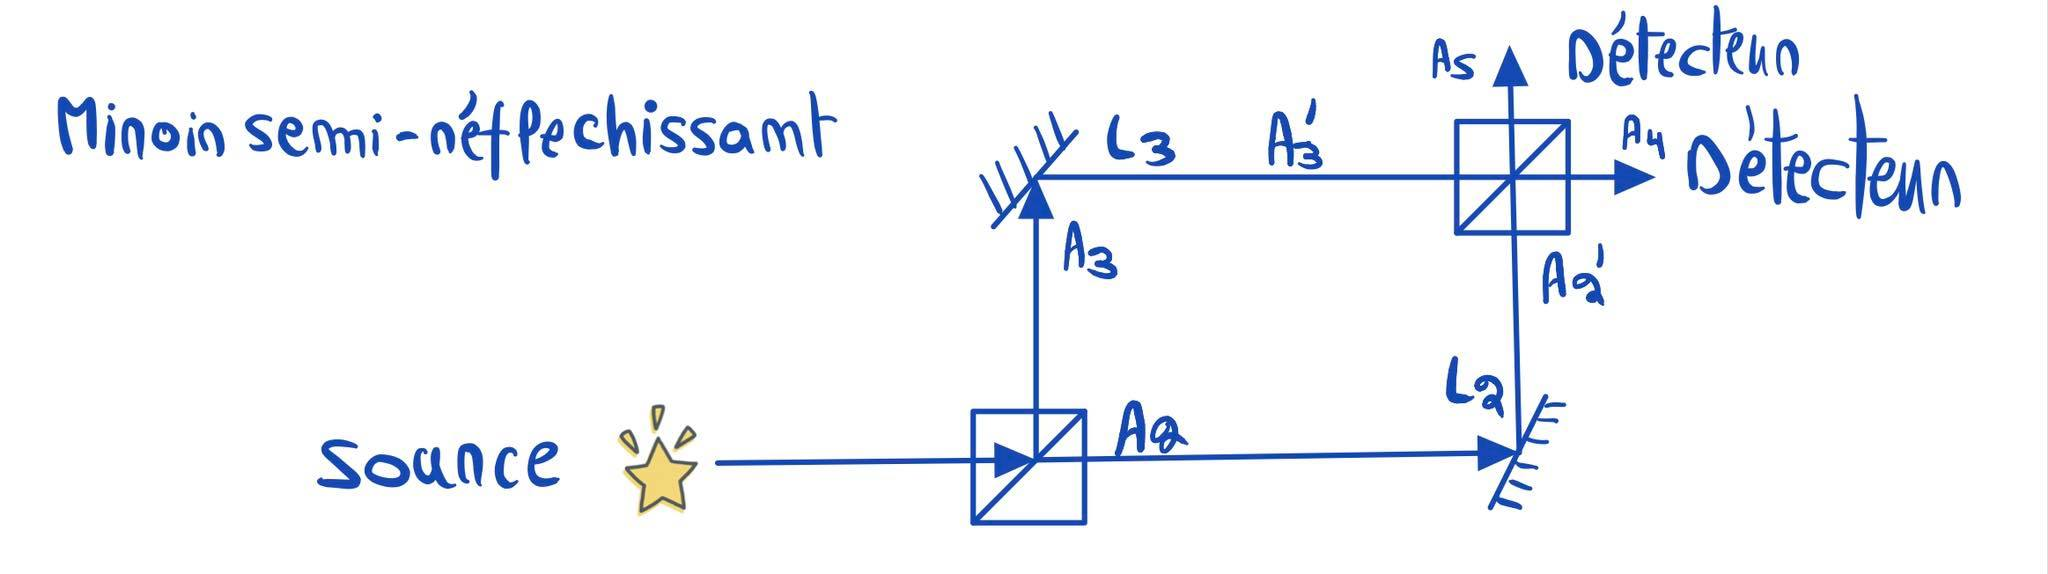
\includegraphics[width=0.80\textwidth]{Mach-Zehnder.png}
\caption{Représentation du principe de l'interféromètre de Mach-Zehnder. Notons que les longueurs $L_i$ représentent la longueur totale du trajet dans le chemin $i$ suivit.}
\label{Mach-Zehnder}
\end{figure}
\end{center}

\subsection{Brève description des détecteurs}
Au niveau des détecteurs, plusieurs chemins sont possibles, comme l'illustre l'image ci-contre.
\begin{center}
\begin{figure}[h]
\centering
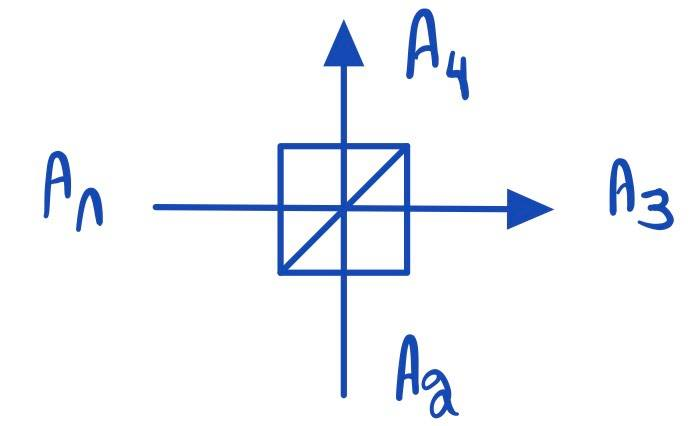
\includegraphics[width=0.50\textwidth]{bean.png}
\caption{Les ondes incidentes arrivants de $A_1$ et $A_2$ poursuivent leur chemin, respectivement en $A_3$ et $A_4$.}
\label{Interferometre}
\end{figure}
\end{center}
Nous avons un miroir semi-transparant. Nous envoyons dessus par le port 1 un faiseau de lumière d'amplitude $A_1$, et d'intensité $I_1 = \norm{A_1}^2$ ; par le port 2, nous envoyons un faisceau d'amplitude $A_2$ et d'intensité $I_2 = \norm{A_2}^2$. \emph{En supposant qu'il n'y a pas de pertes}, nous avons que la somme des intensités entrantes est égale à la somme des intensités sortantes : $I_1 + I_2 = I_3 + I_4$. Puisque les équations de l'électromagnétisme sont linéaires, nous avons $A_3 = \alpha A_1 + \beta A_2$, pour tout $\alpha,\beta\in\mathbb{C}$. Nous pouvons facilement mesurer les valeurs absolues de ces coefficients. En posant $A_2 = 0$, nous pouvons mesurer $I_3$ ; nous trouverons $\norm{\alpha}^2$.\\

Partons de la description d'une onde plane. Nous aurons
\begin{subequations}
\begin{equation}
A_1 (t) = A_1e^{-i\omega t},
\end{equation}
\begin{equation}
A_2 (t) = A_2e^{-i\omega t},
\end{equation}
\end{subequations}
pour les ondes incidentes, ainsi que
\begin{subequations}
\begin{equation}
A_3 (t) = cA_1e^{-i\omega t} + i s A_2e^{-i\omega t}
\end{equation}
\begin{equation}
A_4 (t) = c A_2e^{-i\omega t} + i sA_1e^{-i\omega t}
\end{equation}
\end{subequations}
pour les ondes sortantes. La discussion précédente nous permet de choisir un des coefficients - soit $\norm{c}^2$ - en choissisant le miroir semi-transparent. Le coefficient $\norm{s}^2$ est alors fixé par
\begin{equation}
\norm{c}^2 + \norm{s}^2 = 1.
\end{equation}
Il nous reste une liberté de phase : nous pouvons redéfinir la phase de $A_1 = e^{i \Phi}A'_1$, et de même pour $A_2, A_3$ et $A_4$. Il s'agit d'une question de convention.
\begin{remark} Par convention, les ondes transmises ne subissent aucun déphasage, là où les ondes réfléchies bénéficient d'un déphasage de $\frac{\pi}{2}$. D'autres conventions sont possibles.\end{remark}

\begin{remark} Nous pouvons prendre $c = \cos\theta$ et $s = \sin\theta$ pour un argument $\theta$, ce qui explique la notation utilisée. \end{remark}

\subsection{Lumière classique}
Pour simplifier, prenons $c = \frac{1}{\sqrt{2}} = s$. Notons que nous pouvons introduire un facteur $e^{ikL}$ tenant compte de la distance parcourue, i.e. un point en $x = 0$ peut-être décrit par $A(t) = Ae^{-i\omega t}$ et un point en $x = L$ peut-être décrit par $A'(t) = Ae^{-i\omega t}e^{ikL}$. Notre détecteur repère le courant électrique $I(t)$ selon $I(t) = e\norm{A(t)}^2$ - soit 
\begin{align*}
A(t) &= Ae^{-i\omega t}	&I_{0} = \norm{A(t_0 = 0)}^2 = \norm{A}^2.
\end{align*}
Nous avons alors que
\begin{align*}
A_2 (t) &= \frac{A(t)}{\sqrt{2}}	&A_3 (t) = i\frac{A(t)}{\sqrt{2}}
\end{align*}
En particulier, nous pouvons écrire les chemins $A_2'$ et $A_3'$ selon:
\begin{subequations}
\begin{align}
A'_2 (t) &= A_2 (t)e^{ikL_2}	&A'_3 (t) = A_3 (t)e^{ikL_3}
\end{align}
\text{De même, les chemins $A_4$ et $A_5$ s'écrivent:}
\begin{align}
A_4 &= \frac{1}{\sqrt{2}} (A'_3 + iA'_2) = i\frac{A(t)}{2} (e^{ikL_3} + e^{ikL_2})		&A_5 = \frac{A(t)}{2} (e^{ikL_2} - e^{ikL_3})  
\end{align}
\end{subequations}
En introduisant le terme $\Delta \Phi = kL_3 - kL_2$, nous pouvons conclure que:
\begin{subequations}
\begin{align}
I_4 &= \frac{\norm{A}^2}{4} \norm{e^{ikL_2} + e^{ikL_3}}^2 = \norm{A}^2 \cos^2 \frac{k(L_3-L_2}{2} = \norm{A}^2 \cos^2 \frac{\Delta\Phi}{2}\\
I_5 &= \norm{A}^2 \sin^2 \frac{\Delta \Phi}{2}
\end{align}
\end{subequations}
Remarquons que $I_4+I_5 \doteq I_{0}$ - soit $I_0 = \norm{A}^2$, comme prévu. Nos calculs tiennent, donc.
\subsection{Lumière quantique}
Le photon peut suivre plusieurs chemin simultanément : par superposition, nous écrivons l'état comme
\begin{equation}
\ket{\Psi} = \alpha\ket{1}+\beta\ket{2}+\gamma\ket{3}
\end{equation}
Où $\ket{i}$ décrit le photon dans le chemin $i$.\\

Dans un beam splitter tel que décrit par \eqref{Interferometre}, nous décrivons alors les transitions
\begin{align}
\ket{1} &\rightarrow c\ket{3} + is\ket{4},\\
\ket{2} &\rightarrow is\ket{3} + c\ket{4}.
\end{align}
Cette transition est décrite par la matrice  $\begin{pmatrix}
c & is\\
is & c
\end{pmatrix}$, unitaire.\\

Soit une mesure dans la base $\ket{1},\ket{2}$ ; donnée par l'était $\ket{\Psi} = \alpha\ket{1}+\beta\ket{2}$. Dès lors, les probabilités de détection seront données par $P_1 = \norm{\alpha}^2$ et $P_2 = \norm{\beta}^2$.\\

Il s'ensuit que la decription de l'interféromètre \ref{Interferometre} sera la suivante:
\begin{itemize}
\item \textbf{Chemins 2 et 3.}
\begin{equation}
\ket{\Psi} = \frac{1}{\sqrt{2}}\ket{2} + \frac{1}{\sqrt{2}}\ket{3}
\end{equation}
\item \textbf{Chemins 2' et 3'.}
\begin{align}
\ket{\Psi} &= \frac{e^{ikL_2}}{\sqrt{2}}\ket{2'} + \frac{i}{\sqrt{2}}e^{ikL_3}\ket{3'}\\
\end{align}
\item \textbf{Chemins 4 et 5.}
\begin{align}
\ket{\Psi} &= \frac{1}{2} (e^{ikL_2} - e^{ikL_3})\ket{5} + \frac{i}{2}(e^{ikL_2} + e^{ikL_3})\ket{4}
\end{align}
\end{itemize}
Dès lors,nous avons que les probabilités de détections en 4 et en 5 seront:
\begin{align}
P_4 &= \cos^2 \frac{\Delta \Phi}{2}\\
P_5 &= \sin^2 \frac{\Delta \Phi}{2}
\end{align}
\emph{Le photon est simultanément dans les chemins 2 et 3.}\\

Remarquons que si nous supprimons le beam splitter à la fin, les probabilités de présence se réduisent à
\begin{equation}
P_4 = \frac{1}{2} = P_5
\end{equation}

Les \emph{delayed choice experiment} (Wheeler, 1978) - qui consistent à enlever/remettre le beam splitter, ou à changer la phase $\Delta\Phi$ après que le photon soit entré dans l'interféromètre - nous apprennent que \textbf{toute interprétation ou l'on suppose que le photon "sait à l'avance ce qu'il doit faire", ne tient pas.}

\section{Oscillations de neutrinos}
Les neutrinons sont des particules neutres, intéragissant très faiblement avec la matière. Elle fût prédite par Pauli pour expliquer le spectre des $e^-$ dans la désintégration du $\beta : n \Rightarrow p^+ + e^- + \nu$.

\section{MASER $NH_3$}
Dans cette section, nous allons discuter d'un appareil fort pratique: le MASER\footnote{Acronyme anglais pour 'Microwave Amplicifaction by Stimulated Emission of Radiation'.} d'ammonium $NH_3$ ; l'un des ancêtres des LASER\footnote{Acronyme anglais pour 'Light Amplification by Stimulated Emission of Radiation'.}

\section{Spin $\frac{1}{2}$}
Nous voyons en cette section une très brève introduction à la quantification du moment angulaire en Mécanique Quantique. Pour ce faire, introduisons le $\mathcal{G}$roupe des $\mathcal{R}$otations.

Considérons l'ensemble des matrices $R \in \mathbb{R}^{3\times 3}$ telle que $R^TR = \mathbb{I}$. Si $\bm{n}$ est un vecteur unitaire de $\mathbb{R}^3$ et $\theta$ un angle, alors $R(\theta,\bm{n}$) est la rotation (en son sens anti-horlogique) autour de l'axe $\bm{n}$ d'angle $\theta$.
\begin{align*}
R(\theta,x) &= \begin{pmatrix}
1 & 0 & 0\\
0 & \cos\theta & -\sin\theta\\
0 & \sin\theta & \cos\theta
\end{pmatrix} = \exp (i\theta L_x)			&L_x = \begin{pmatrix}
0 & 0 & 0\\
0 & 0 & i\\
0 & -i & 0
\end{pmatrix}\\
R(\theta,y) &= \begin{pmatrix}
\cos\theta & 0 & \sin\theta\\
0 & 1 & 0\\
-\sin\theta & 0 & \cos\theta\\
\end{pmatrix} = \exp(i\theta L_y)		&L_y = \begin{pmatrix}
0 & 0 & -i\\
0 & 0 & 0\\
i & 0 & 0
\end{pmatrix}\\
R(\theta,z) &= \begin{pmatrix}
\cos\theta & -\sin\theta & 0\\
\sin\theta & \cos\theta & 0\\
0 & 0 & 1
\end{pmatrix} = \exp(i\theta L_z)		&L_z = \begin{pmatrix}
0 & i & 0\\
-i & 0 & 0\\
0 & 0 & 0
\end{pmatrix}
\end{align*}
Nous avons alors que $R(\theta,\bm{n}) = \exp (i\theta\bm{n}\cdot\bm{L})$, où $\bm{n}\cdot\bm{L} = n_iL_i$. Les vecteurs $L_x,L_y,L_z$ sont appelés les \emph{générateurs du $\mathcal{G}$roupe des $\mathcal{R}$otations}.\\

En physique, de nombreux objets (et non pas seulement les vecteurs) sont invariants ou se transforment sous l'effet d'une rotation. Une autre représentation du $\mathcal{G}$roupe des $\mathcal{R}$otations est l'ensemble des 3 opérateurs $J_x,J_y,J_z$ tels que $[J_x,J_y] = J_z$ (ainsi que toute permutation cyclique de cela) et tel que, sous toute rotation d'angle $\theta$ autour de $\bm{n}$, un état $\ket{\Psi}$ se transforme en
\begin{equation}
\ket{\Psi} \rightarrow \exp(i\theta\bm{n}\cdot\bm{J})\ket{\Psi}
\end{equation}

\begin{exemple}Les opérateurs
\begin{itemize}
\item $J_x = yp_z - zp_y$
\item $J_y = zp_x - xp_z$
\item $J_z = xp_y - yp_x$
sont des exemples de représentation du $\mathcal{G}$roupe des $\mathcal{R}$otations.
\end{itemize}
\end{exemple}
Un système est invariant par rotation lorsque
\begin{align*}
\exp (-itH) \exp (i\theta \bm{n}\cdot\bm{J})\ket{\Psi} &= \exp (i\theta \bm{n}\cdot\bm{J})\exp (-itH) \ket{\Psi}			&\forall \ket{\Psi},\forall \bm{n},\theta,t
\end{align*}
Cela revient à dire que \emph{faire une rotation} et ensuite \emph{évoluer dans le temps} est identique à \emph{évoluer dans le temps} et puis \emph{faire une rotation}.\\
\begin{lemma} Pour $\theta$ et $t$ infinitésimaux, nous avons que 
\begin{equation}
[H,J_x] = [H,J_y] = [H,J_z] = 0
\end{equation}
\end{lemma}
Les conséquences en sont nombreuses. Nous avons notamment alors que:
\begin{enumerate}
\item Si $\ket{\Psi(t)}$ est une solution de l'équation de Schrödinger \eqref{Postulat 4}, alors $\braket{\Psi(t)|J_x|\Psi(t)} = \braket{\Psi(0)|J_x|\Psi(0)}$.
\item Si $<ket{\Psi}$ est un vecteur propre de $J_x$,
\begin{equation}
J_x\ket{\Psi} = j\ket{\Psi}
\end{equation}
alors $\ket{\Psi(t)} = \exp (-iHt)\ket{\Psi}$ est aussi un vecteur propre de $J_x$.
\end{enumerate}
Le $\mathfrak{T}$héorème d'$\mathfrak{E}$mmy $\mathfrak{N}$öther nous apprend que la grandeur conservée par la symmétrie de rotation est le moment angulaire.

\subsection{Quantification du moment angulaire}
\begin{theorem}
Soit $[J_x,J_y] = iJ_z$. Nous avons alors que les valeurs propres de $J_z$ est un demi-entier: $0,\frac{1}{2}, 1, \frac{3}{2}, ...$.
\begin{equation*}
J_z \ket{\Psi} = m\ket{\Psi}
\end{equation*}
\end{theorem}
\begin{theorem}
Il existe une représentation non triviale du $\mathfrak{G}$roupe des $\mathfrak{R}$otations par des matrices $d\times d$. Dans ce cas, $J_z = -\frac{d}{2}, -\frac{d}{2}+1,...,+\frac{d}{2}$.
\end{theorem}
\begin{exemple}
Le cas le plus simple est celle des matrices de Pauli (matrices $2\times 2$):
\begin{center}
\begin{tabular}{c|c|c}
$\sigma_x = \begin{pmatrix}
0 & 1\\
1 & 0
\end{pmatrix}$ & $\sigma_x = \begin{pmatrix}
0 & -i\\
i & 0
\end{pmatrix}$ & $\sigma_x = \begin{pmatrix}
1 & 0\\
0 & -1
\end{pmatrix}$\\
$J_x = \frac{1}{2}\sigma_x$ & $J_y = \frac{1}{2}\sigma_y$ & $J_z = \frac{1}{2}\sigma_z$
\end{tabular}
\end{center}
Nous pouvons vérifier que les différentes relations démontrées ci-dessus sont respectées (exercice).
\end{exemple}

\color{red}
\textbf{A TERMINER}

\end{document}